\section{TMC4671}\label{Appendix:TMC4671}

\subsection{Standard-Schaltkreis}\label{Appendix:Schaltung_TMC4671}

\begin{figure}[H]
	\centering
	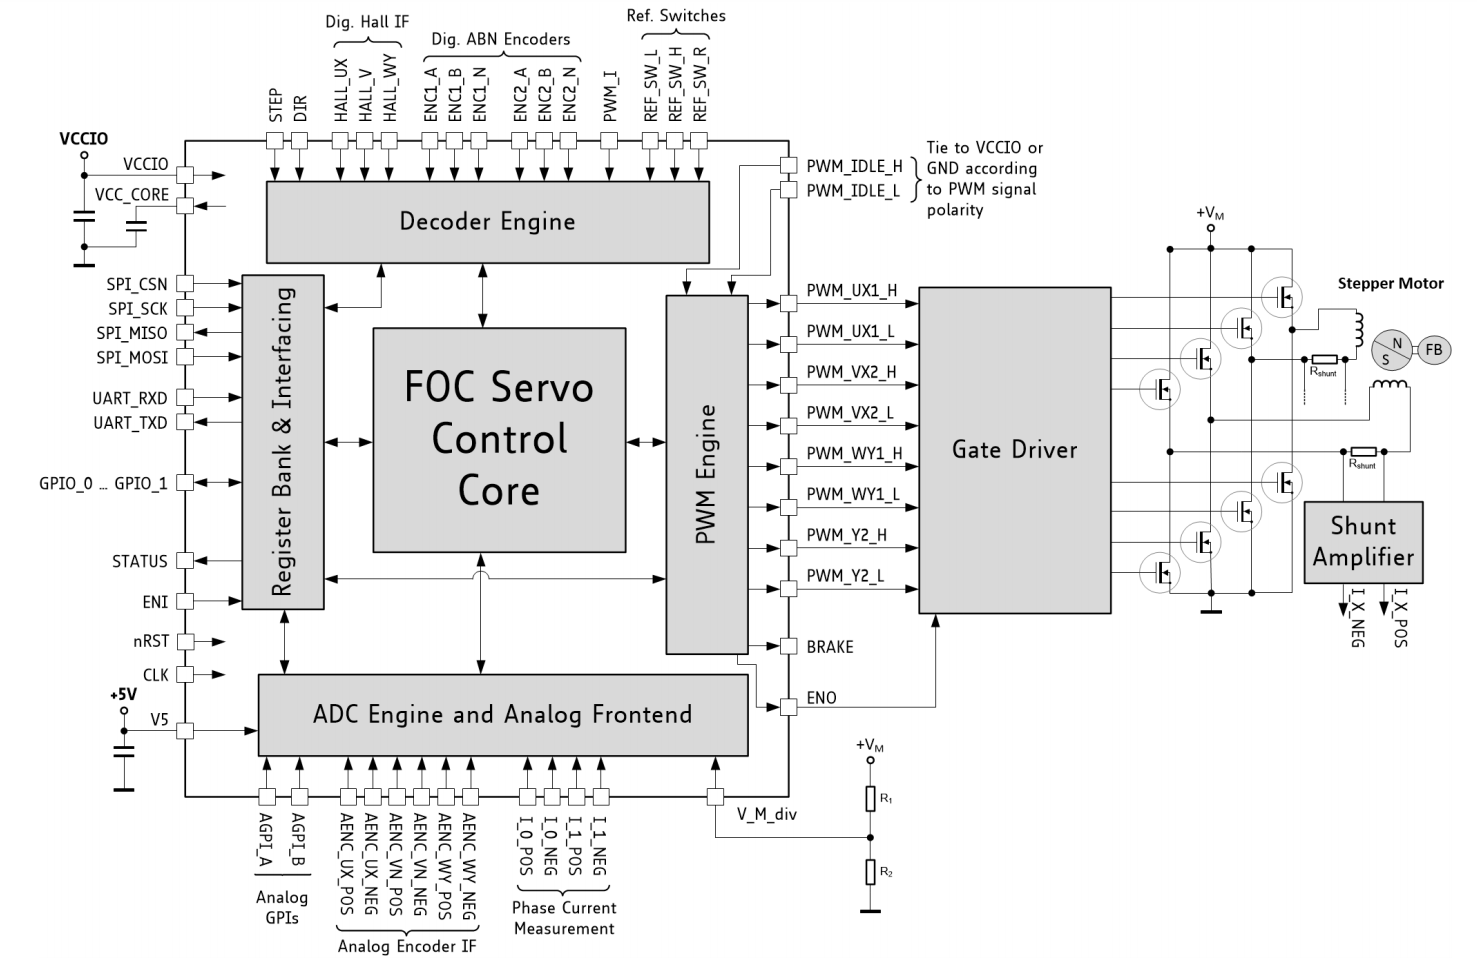
\includegraphics[width=0.8\textwidth]{graphics/Standard_Application_Cirquit_TMC4671}
	\caption{Standard-Anwendungs-Schaltung. \cite[S.138]{trinamicmotion_control_gmbh__co_kg_tmc4671_2019}}
	\label{fig:Schaltung_TMC4671}
\end{figure}

\subsection{BOB}\label{Appendix:BOB}

\begin{figure}[H]
	\centering
	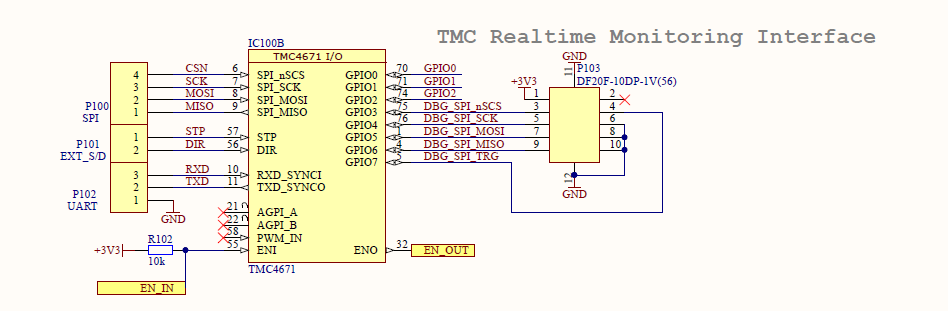
\includegraphics[width=\textwidth]{graphics/TMC4671_SPI_BOB_Schematic}
	\caption{SPI-Input des TMC4671-BOB. \cite[S.2]{trinamicmotion_control_gmbh__co_kg_tmc4671-bob_2020}}
	\label{fig:Schema_SPI_FOC_Treiber}
\end{figure} 

\begin{figure}[H]
	\centering
	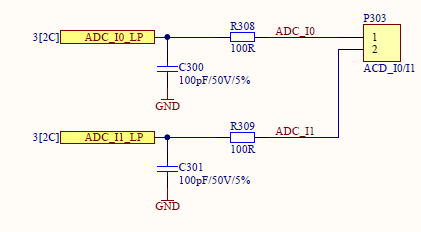
\includegraphics[width=0.5\textwidth]{graphics/TMC4671_Phasenstroeme_BOB_Schematic}
	\caption{Phasenstroeme-Input des TMC4671-BOB. \cite[S.4]{trinamicmotion_control_gmbh__co_kg_tmc4671-bob_2020}}
	\label{fig:Schema_Phasenstroeme_FOC_Treiber}
\end{figure} 

\begin{figure}[H]
	\centering
	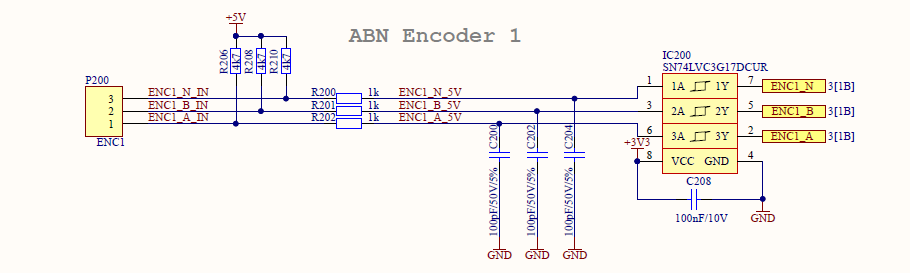
\includegraphics[width=0.7\textwidth]{graphics/TMC4671_ABN_Encoder_BOB_Schematic}
	\caption{ABN-Encoder-Input des TMC4671-BOB. \cite[S.3]{trinamicmotion_control_gmbh__co_kg_tmc4671-bob_2020}}
	\label{fig:Schema_ABN_Encoder_FOC_Treiber}
\end{figure} 

\begin{figure}[H]
	\centering
	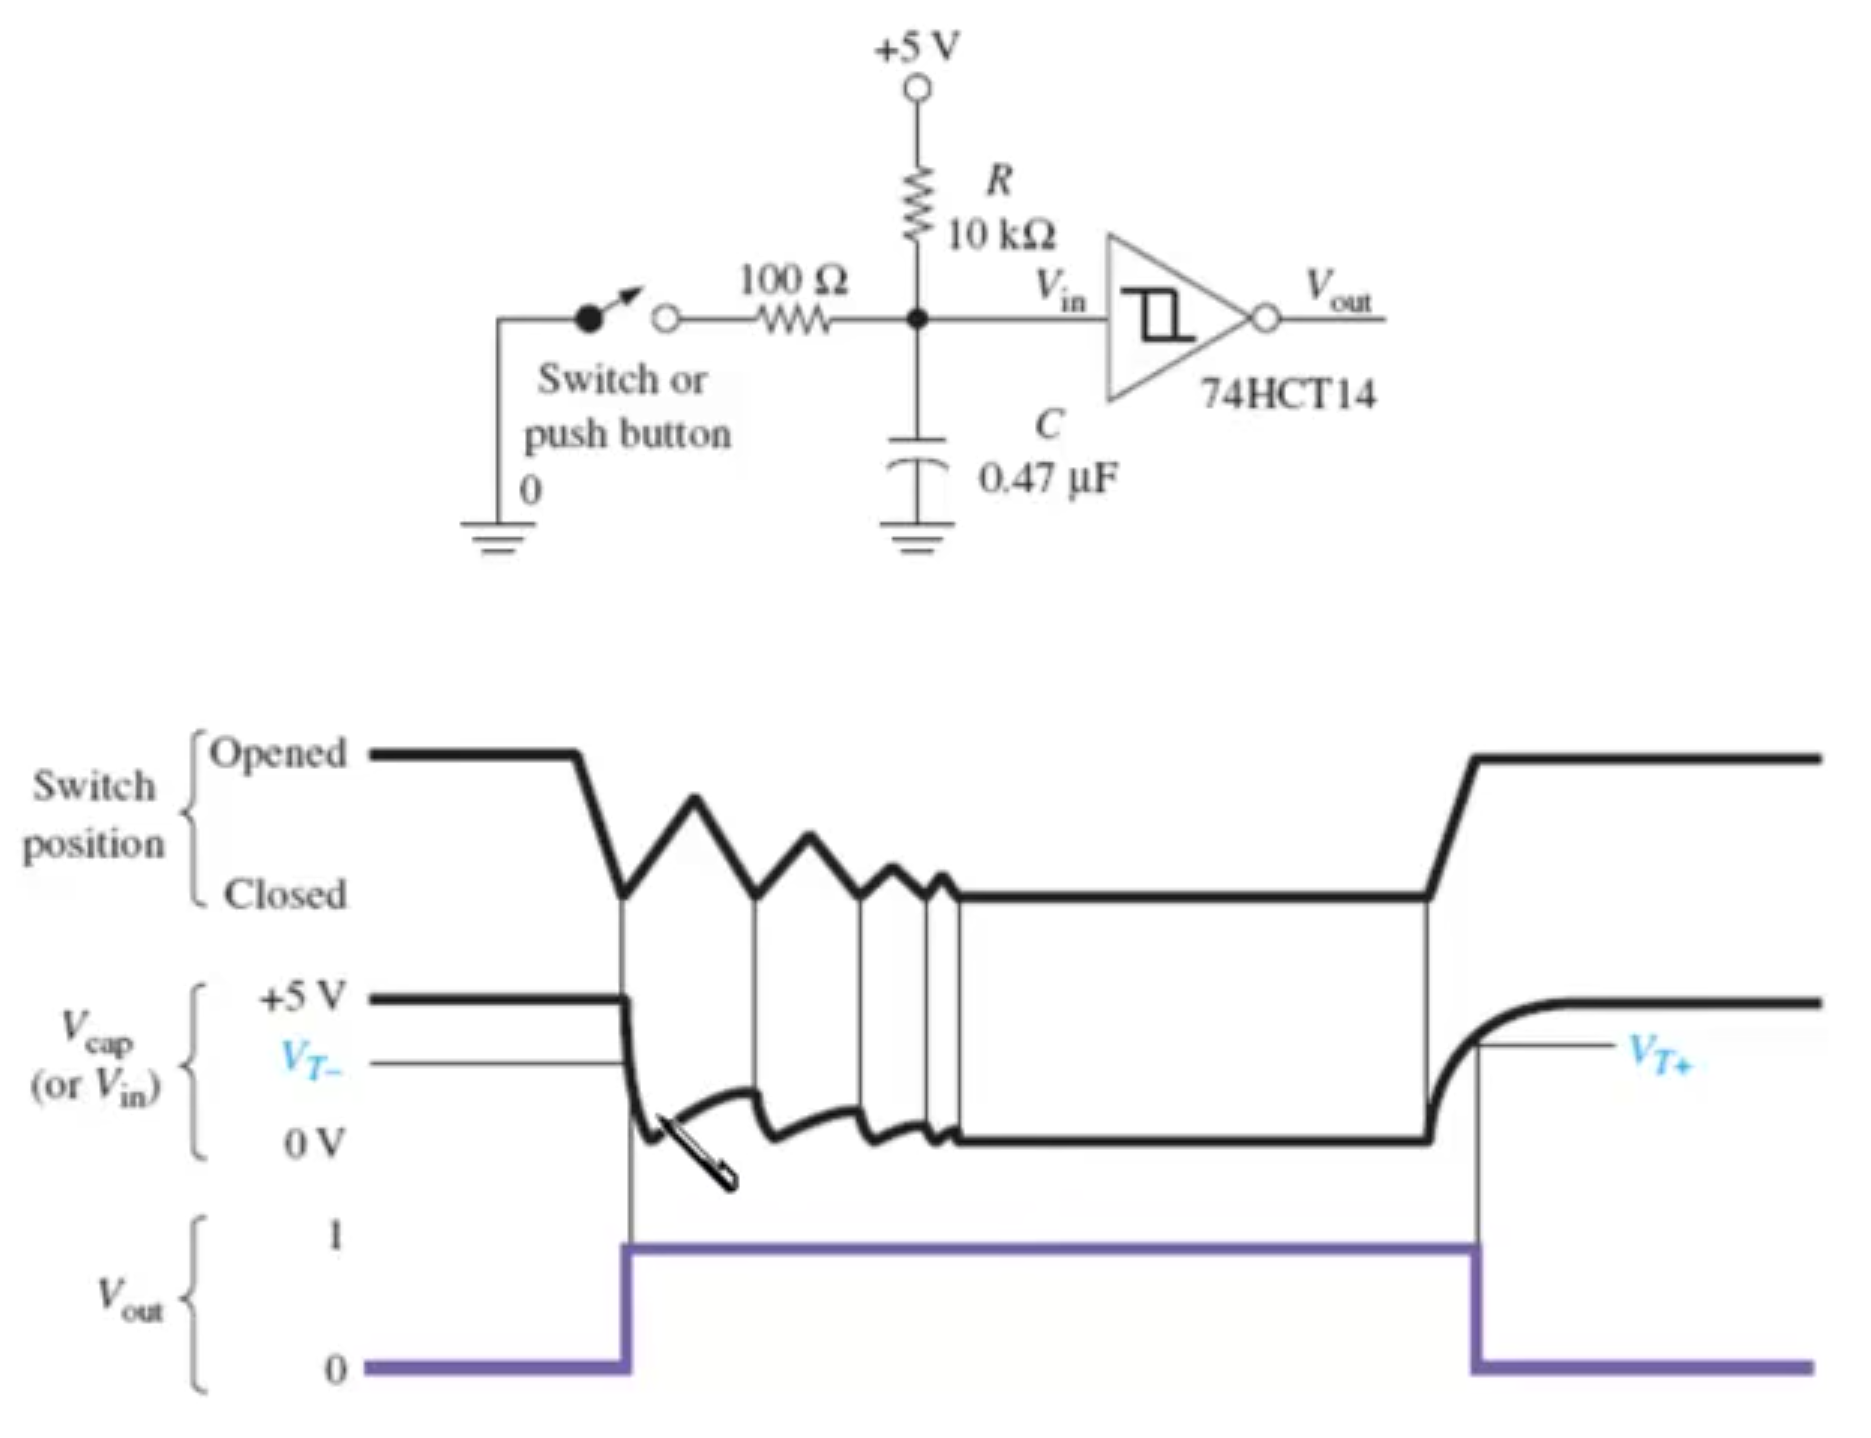
\includegraphics[width=0.7\textwidth]{graphics/Schmitt_Trigger_Debounce}
	\caption{Schmitt-Trigger Debounce-Schaltung. \cite[3:00]{kleitz_sec_2011}}
	\label{fig:Schmitt_Trigger_Debounce}
\end{figure} 

\begin{figure}[H]
	\centering
	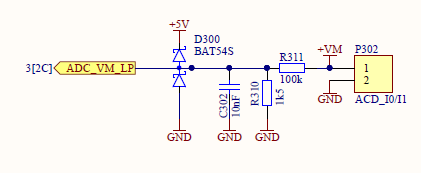
\includegraphics[width=0.7\textwidth]{graphics/TMC4671_Motorspannung_BOB_Schematic}
	\caption{Motorspannung-Input des TMC4671-BOB. \cite[S.4]{trinamicmotion_control_gmbh__co_kg_tmc4671-bob_2020}}
	\label{fig:Schema_Motorspannung_FOC_Treiber}
\end{figure} 

\begin{figure}[H]
	\centering
	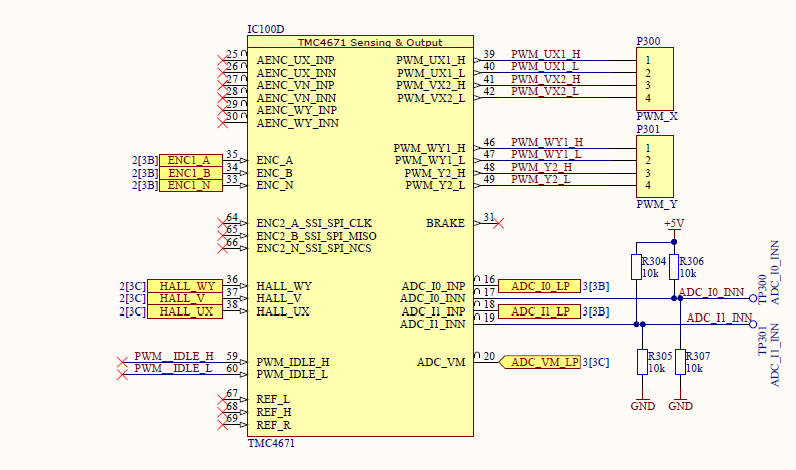
\includegraphics[width=0.7\textwidth]{graphics/TMC4671_PWM_BOB_Schematic}
	\caption{PWM-Output des TMC4671-BOB. \cite[S.3]{trinamicmotion_control_gmbh__co_kg_tmc4671-bob_2020}}
	\label{fig:Schema_PWM_FOC_Treiber}
\end{figure} 

\subsection{Inbetriebnahme}

\subsubsection{Register Openloop}\label{Appendix:TMC4671_Register}

\begin{table}[H]
\begin{tabularx}{\textwidth}{|l|l|l|X|}
\hline
\multicolumn{4}{|c|}{\textbf{TMC4671 Register}}               \\ \hline
\textbf{Nr. }& \textbf{Register-Name   }   & \textbf{Wert }      & \textbf{Was} \\ \hline
\multicolumn{4}{|l|}{\textbf{Motor type \&  PWM configuration}}        \\ \hline
0x17         & PWM\_POLARITIES             & 0x00000000 & MOSFETs polarity ''off''    \\ \hline
0x1B         & MOTOR\_TYPE\_N\_POLE\_PAIRS & 0x00030003 &     \\ \hline
0x18         & PWM\_MAXCNT                 & 0x00000F9F & PWM frequency 25kHz = 100MHz/(3999+1)   \\ \hline
0x19         & PWM\_BBM\_H\_BBM\_L         & 0x00001919 & Break-before-Make-Time[10ns] MOSFET gate control \\ \hline
0x1A         & PWM\_SV\_CHOP               & 0x00000007 & PWM chopper mode: centtered PWM for FOC \\ \hline
\multicolumn{4}{|l|}{\textbf{ADC configuration}}                       \\ \hline
0x0A         & ADC\_I\_SELECT              & 0x24000100 & ADC\_I0\_(RAW), ADC\_I1\_(RAW)    \\ \hline
0x04         & dsADC\_MCFG\_B\_MCFG\_A     & 0x00100010 & (TMCL-IDE)    \\ \hline
0x05         & dsADC\_MCLK\_A              & 0x20000000 & (TMCL-IDE)    \\ \hline
0x06         & dsADC\_MCLK\_B              & 0x00000000 & (TMCL-IDE)    \\ \hline
0x07         & dsADC\_MDEC\_B\_MDEC\_A     & 0x014E014E & (TMCL-IDE)    \\ \hline
0x09         & ADC\_I0\_SCALE\_OFFSET      & 0xFF0080CF & (TMCL-IDE)    \\ \hline
0x08         & ADC\_I1\_SCALE\_OFFSET      & 0xFF008E04 & (TMCL-IDE)    \\ \hline
\multicolumn{4}{|l|}{\textbf{Open loop settings}}                      \\ \hline
0x1F         & OPENLOOP\_MODE              & 0x00000000 & Openloop Phi Direction positive    \\ \hline
0x20         & OPENLOOP\_ACCELERATION      & 0x0000003C & Openloop Phi Beschleunigung = 60    \\ \hline
0x21         & OPENLOOP\_VELOCITY\_TARGET  & 0xFFFFFFFB & Openloop Phi Geschwindigkeit = 5    \\ \hline
\multicolumn{4}{|l|}{\textbf{Feedback selection}}                      \\ \hline
0x52         & PHI\_E\_SELECTION           & 0x00000002 & Phi-E selector = Phi-E Openloop    \\ \hline
0x24         & UQ\_UD\_EXT                 & 0x00000FA0 & FOC q/d = 4000  \\ \hline
\multicolumn{4}{|l|}{\textbf{Switch to open loop velocity mode}}       \\ \hline
0x63         & MODE\_RAMP\_MODE\_MOTION    & 0x00000008 & Modulation gem. UQ/UD ext. \\ \hline
\multicolumn{4}{|l|}{\textbf{Rotate right}}                            \\ \hline
0x21         & OPENLOOP\_VELOCITY\_TARGET  & 0x0000003C & Openloop Phi Geschwindigkeit = 60    \\ \hline
\end{tabularx}
\end{table}

\subsubsection{Setup}\label{Appendix:TMC4671_Setup}


\begin{figure}[H]
	\centering
	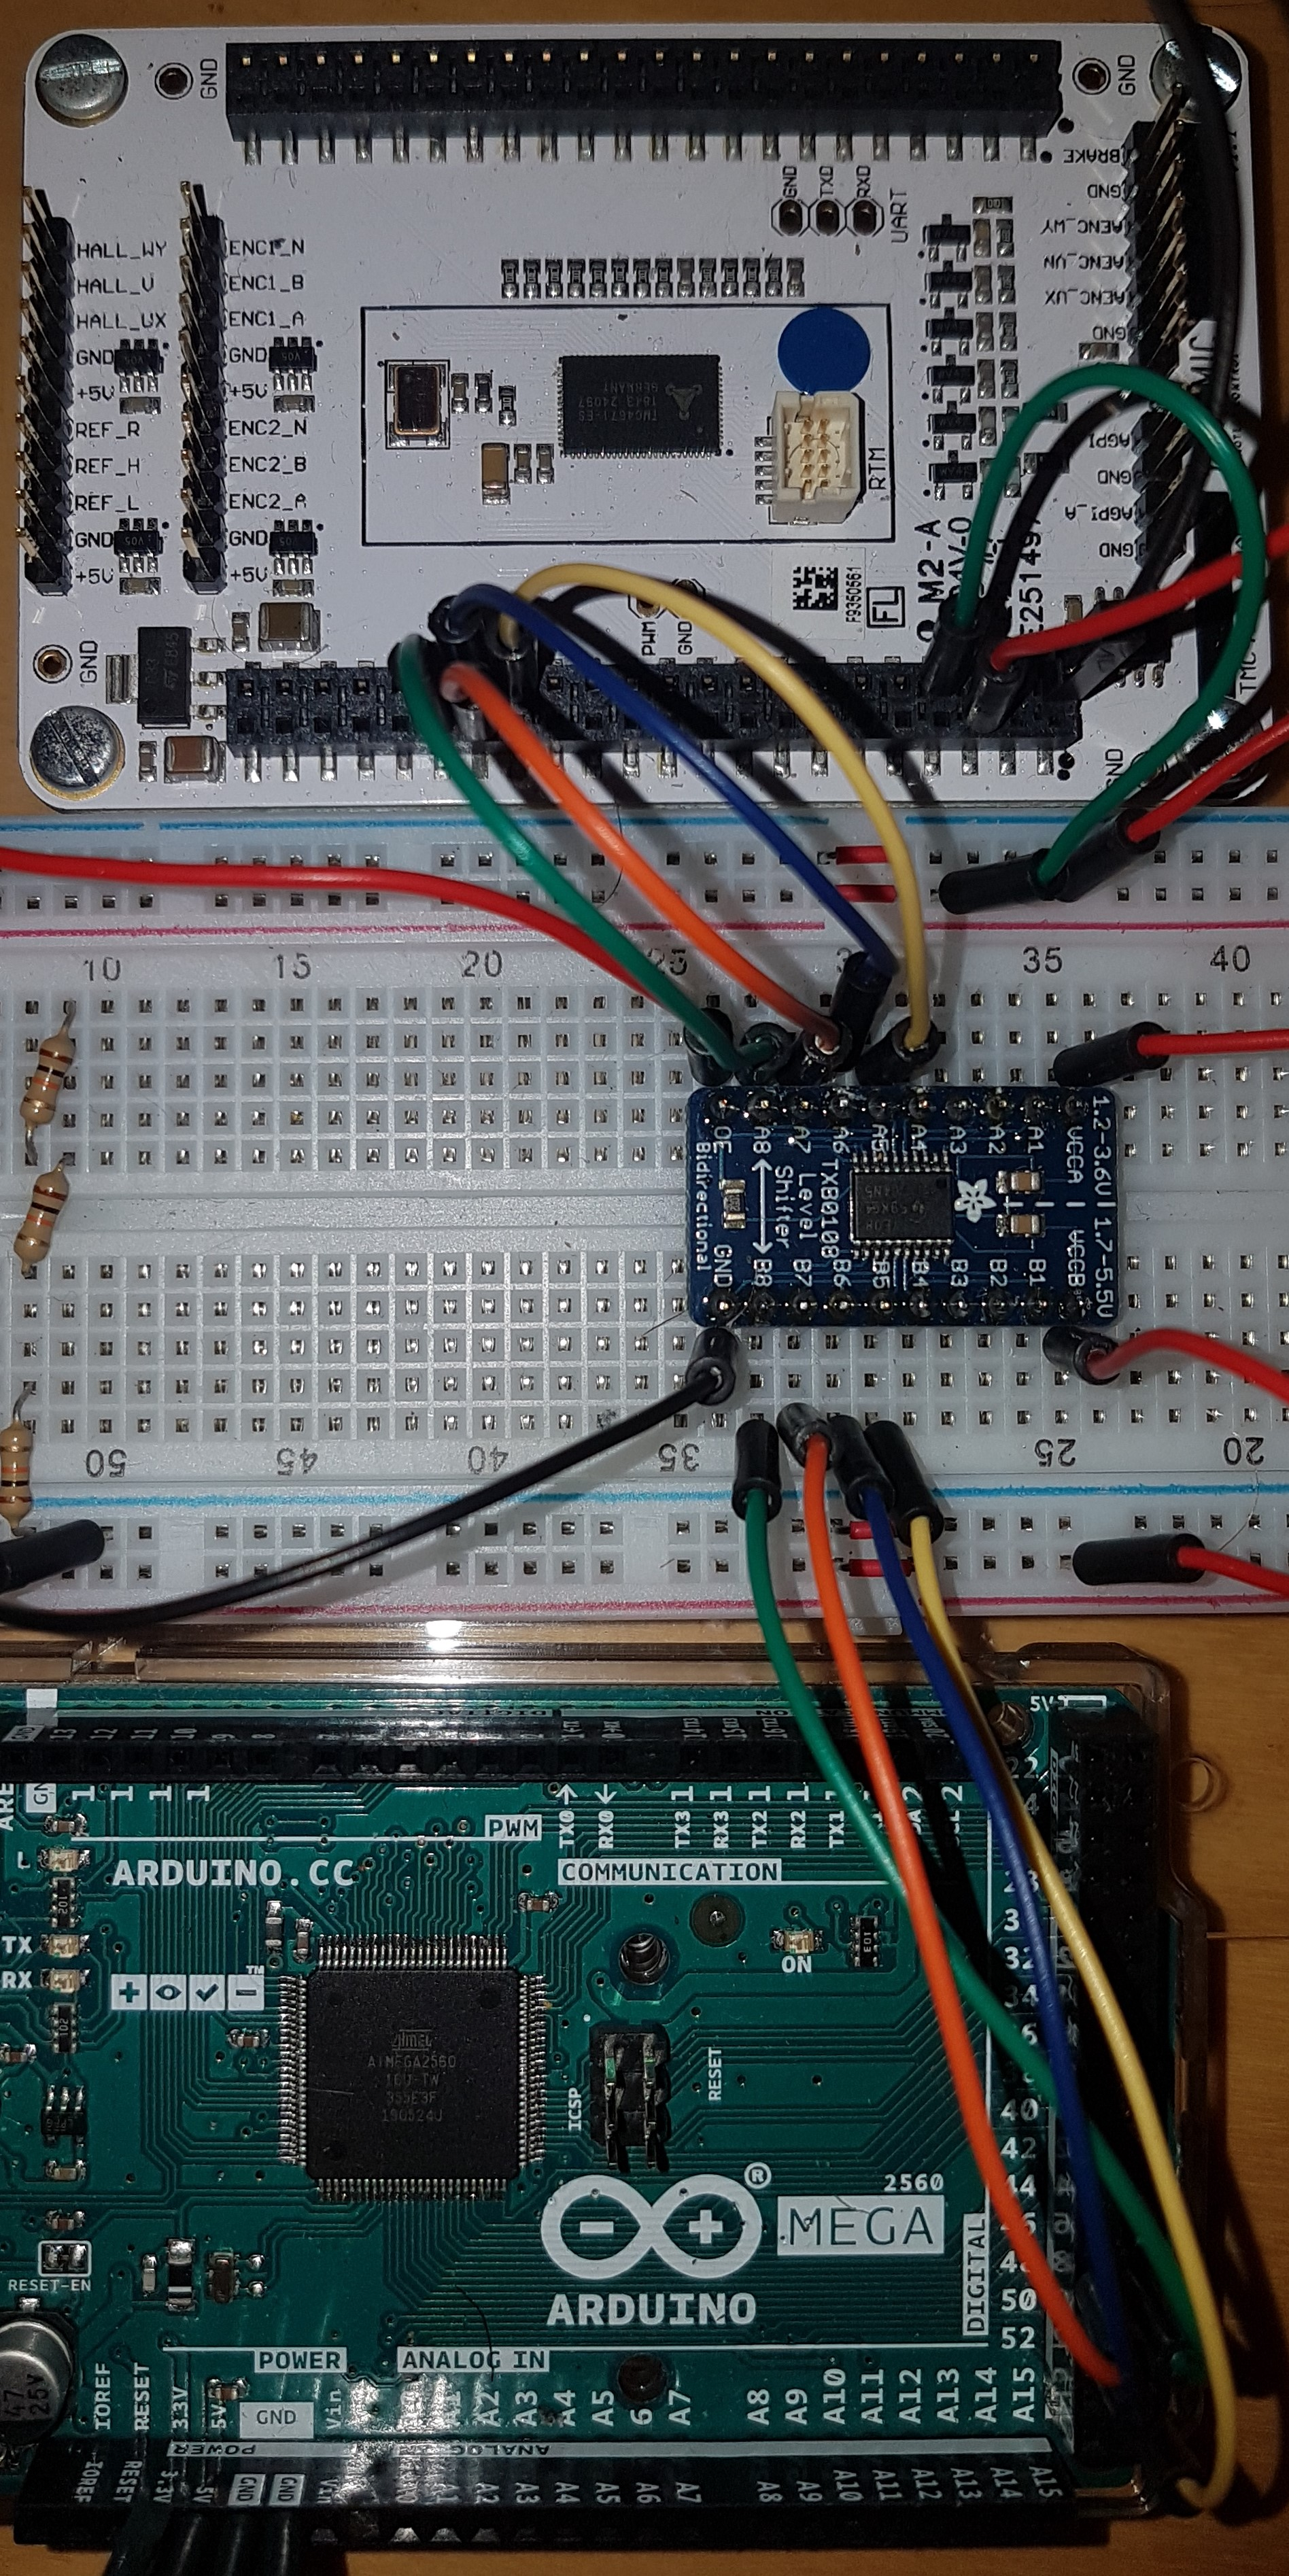
\includegraphics[angle=270,width=\textwidth]{graphics/1_komplett}
	\caption{Gesamtansicht Setup.}
	\label{fig:1_komplett}
\end{figure}

\begin{figure}[H]
	\centering
	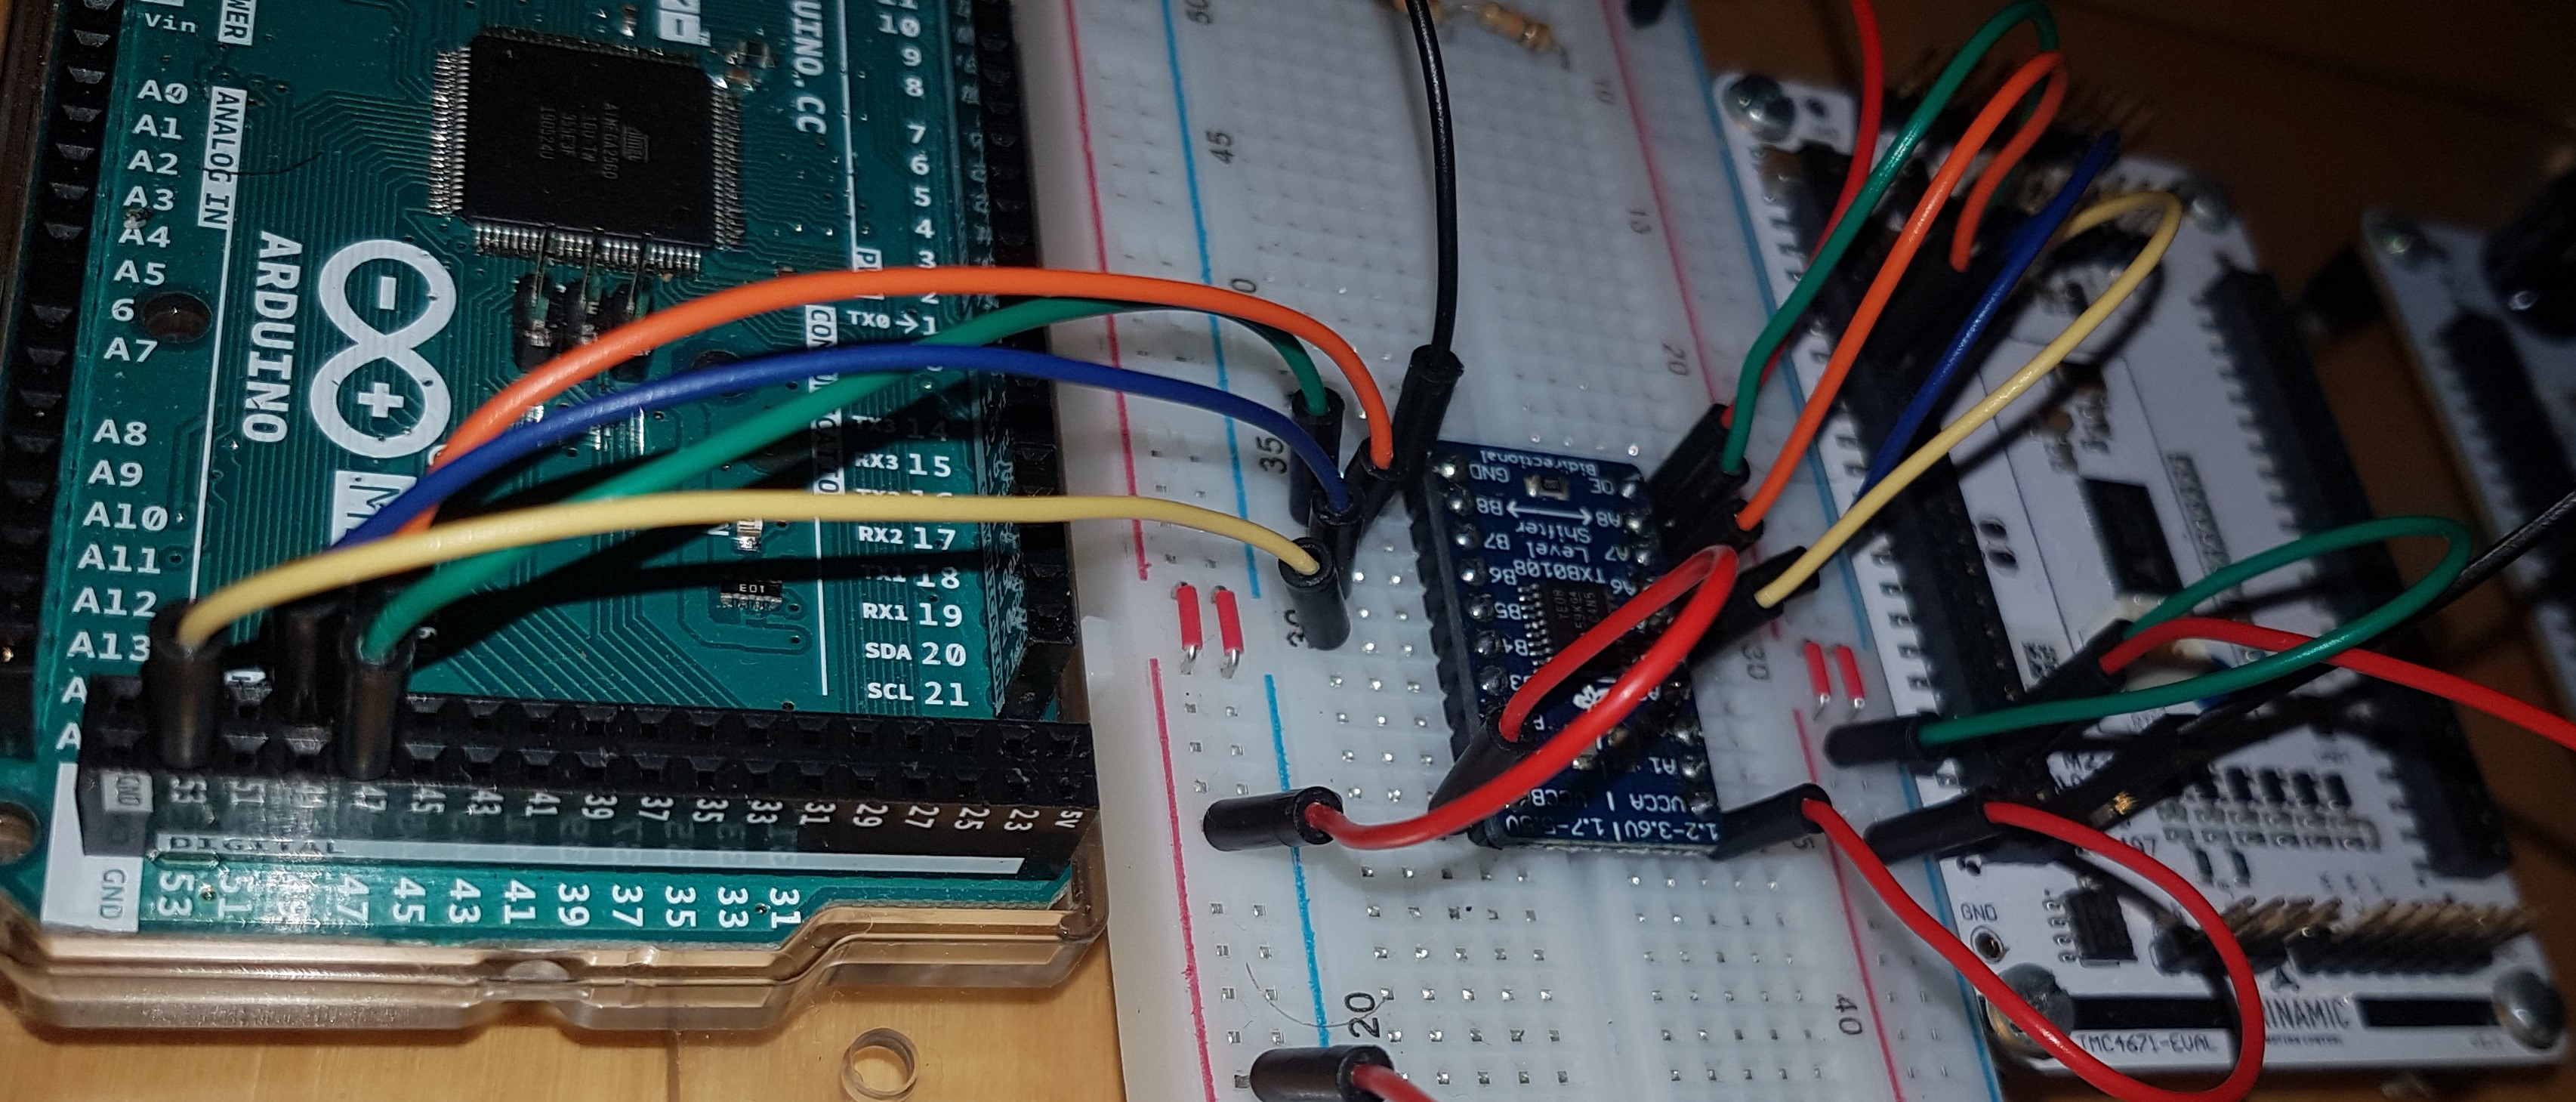
\includegraphics[width=\textwidth]{graphics/1_Arduino}
	\caption{Setup mit Fokus auf Arduino.}
	\label{fig:1_Arduino}
\end{figure}

\begin{figure}[H]
	\centering
	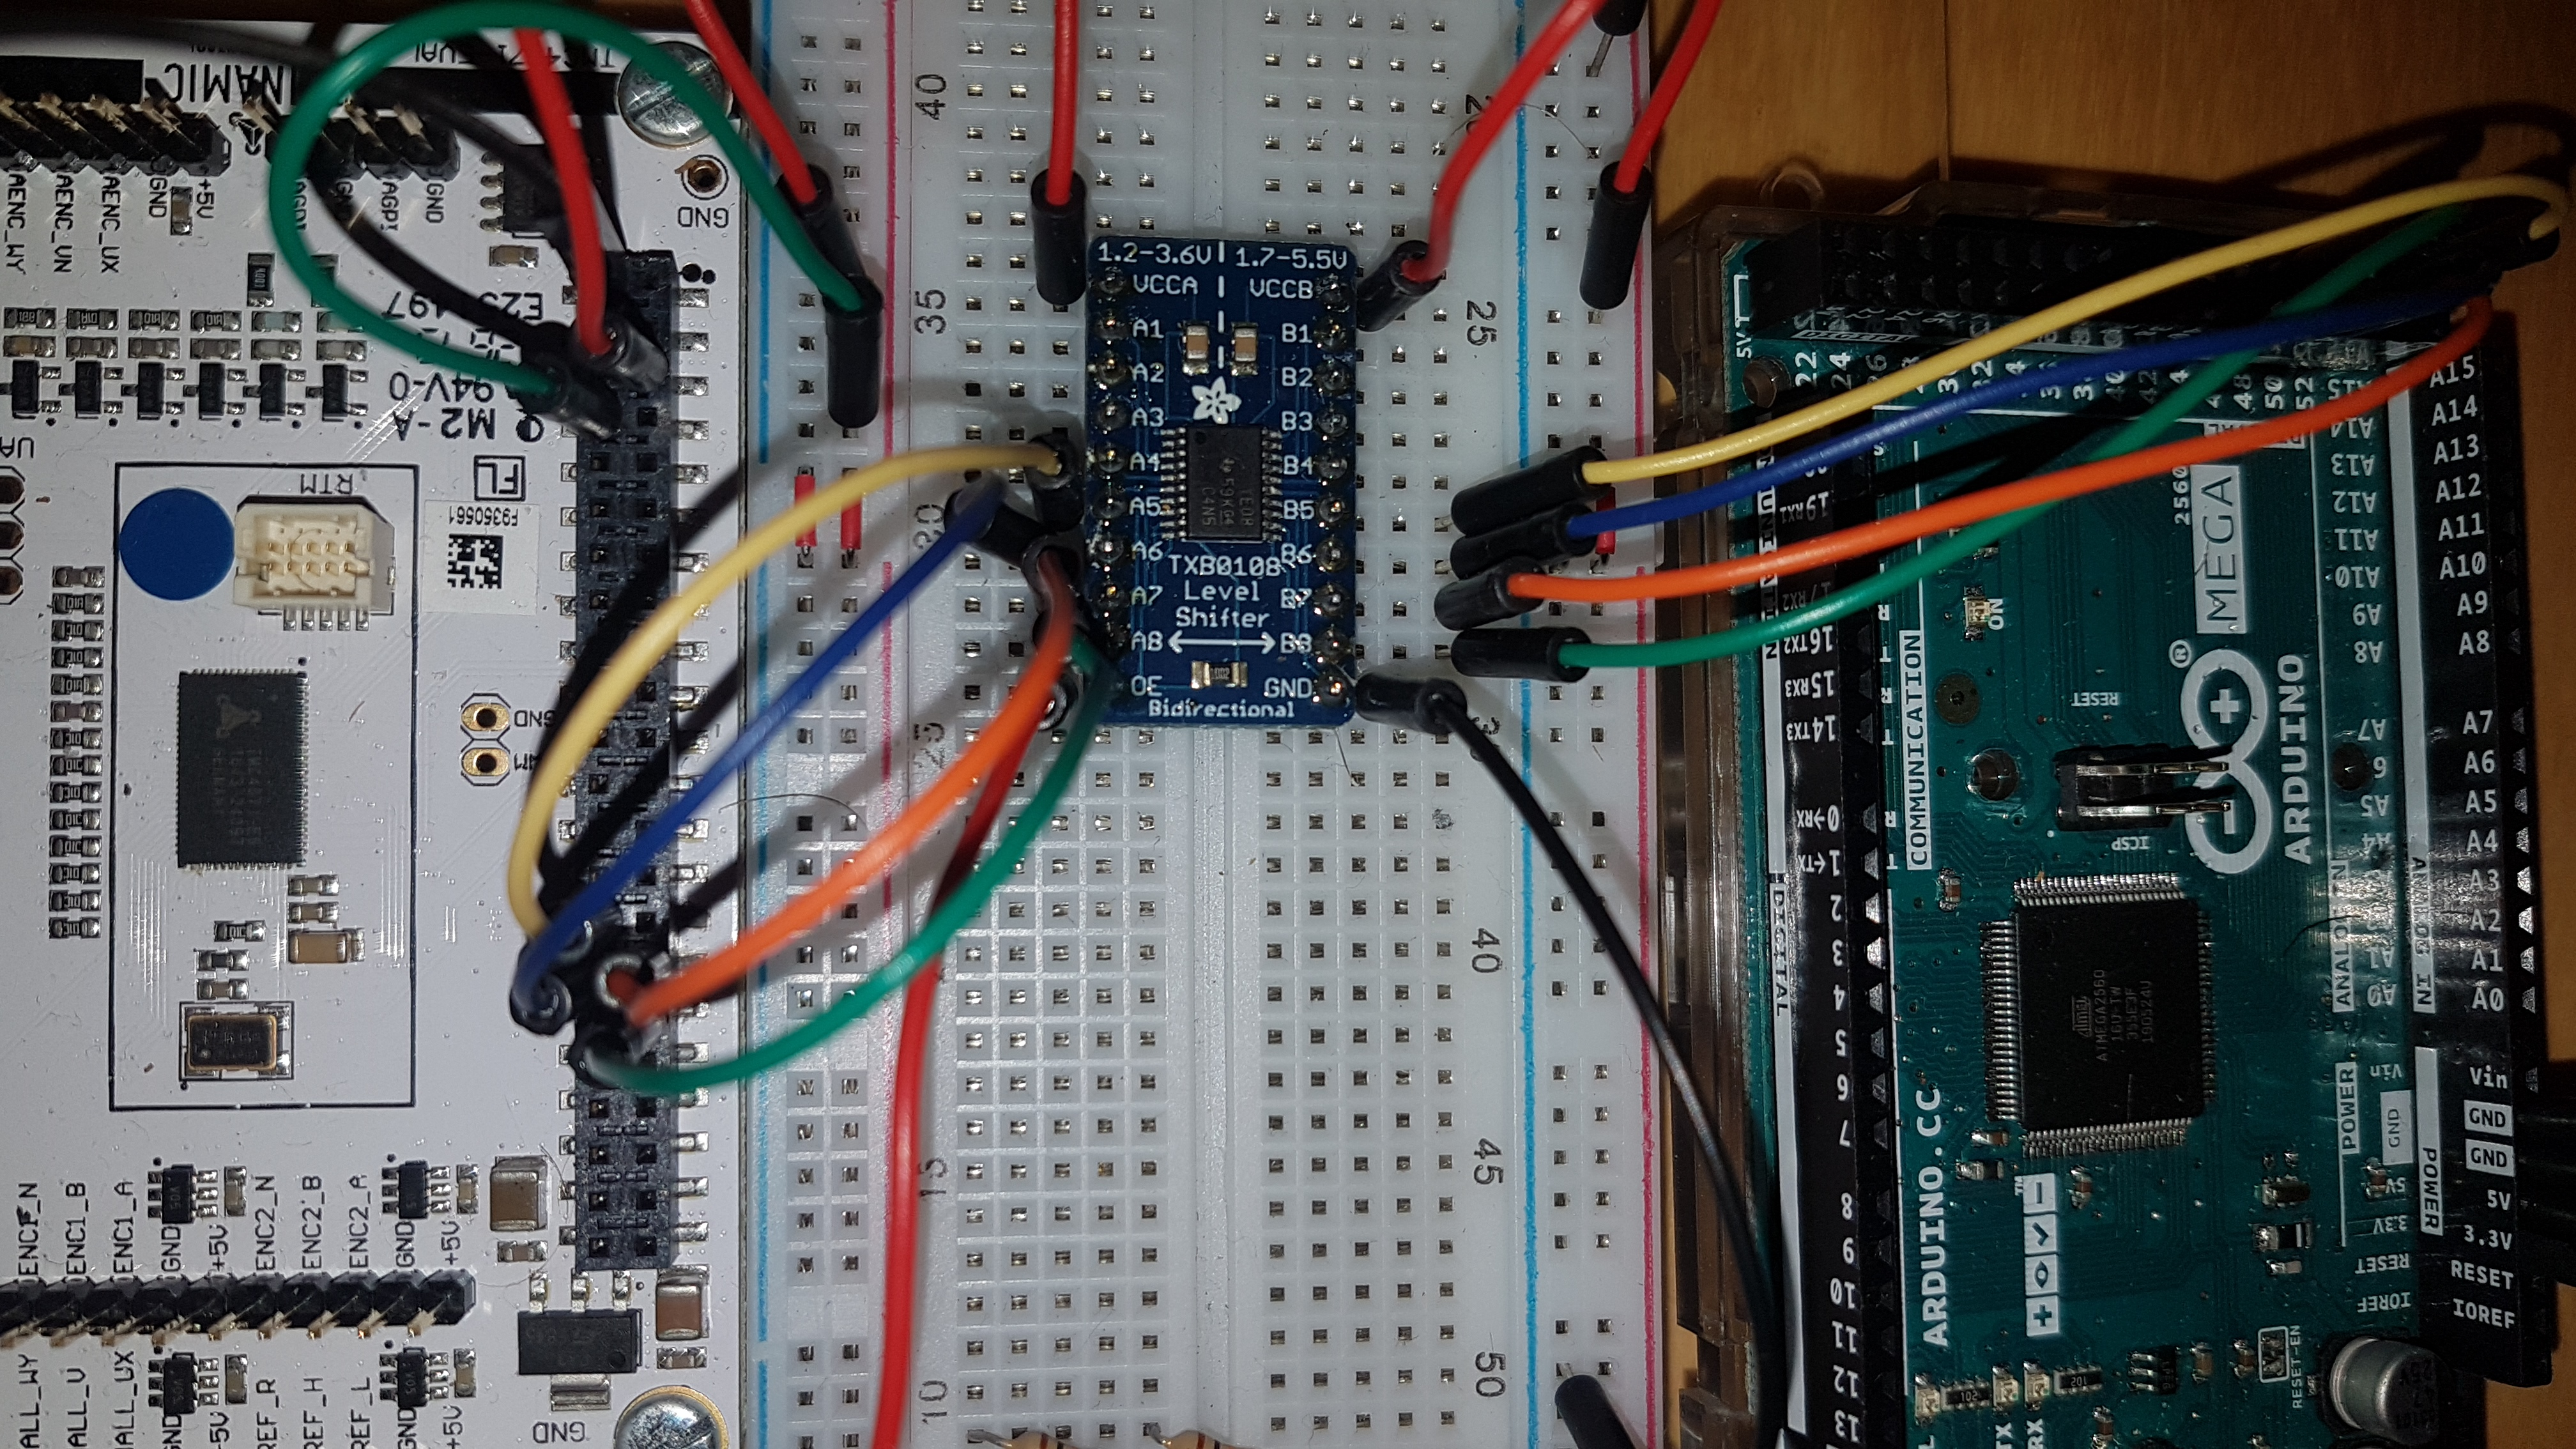
\includegraphics[angle=180,width=\textwidth]{graphics/1_EVAL}
	\caption{Setup mit Fokus auf TMC4674-EVAL.}
	\label{fig:1_EVAL}
\end{figure}

\subsubsection{Inbetriebnahme SPI-Kommunikation}\label{Appendix:TMC4671_SPI}

\begin{figure}[H]
\center
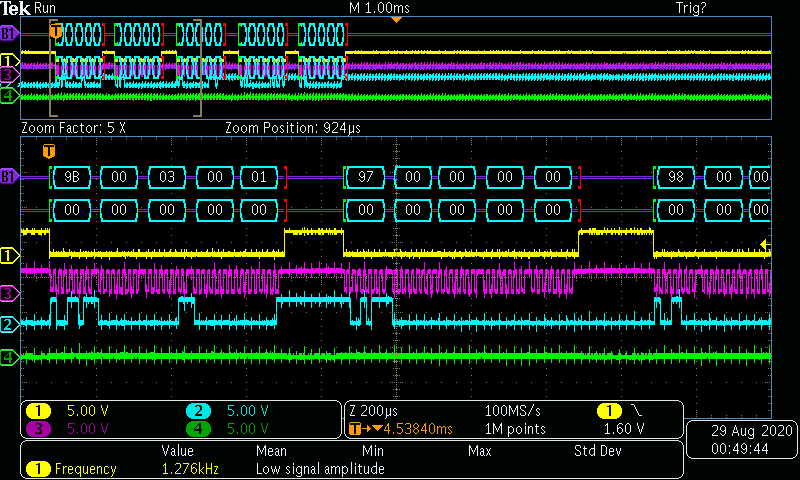
\includegraphics[width = \textwidth]{graphics/TMC4671_Beschreiben_1}
\caption{SPI-Übertragung Write (Hier Motor Pole Pairs).}
\label{fig:TMC4671_Lesen_1}
\end{figure}

\begin{figure}[H]
\center
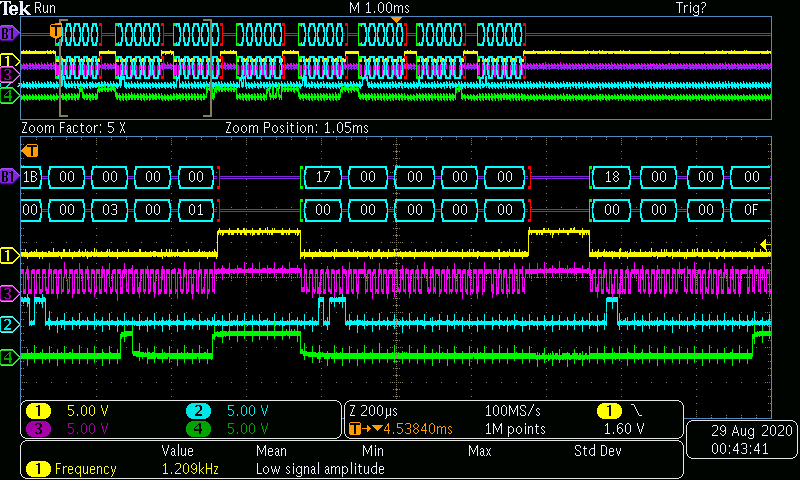
\includegraphics[width = \textwidth]{graphics/TMC4671_Lesen_1}
\caption{SPI-Übertragung Read (Hier Motor Pole Pairs).}
\label{fig:TMC4671_Lesen_1}
\end{figure}
\todo{evt. neue Bilder mit eigenem Aufbau Print}
\newpage
\begin{figure}[H]
\center
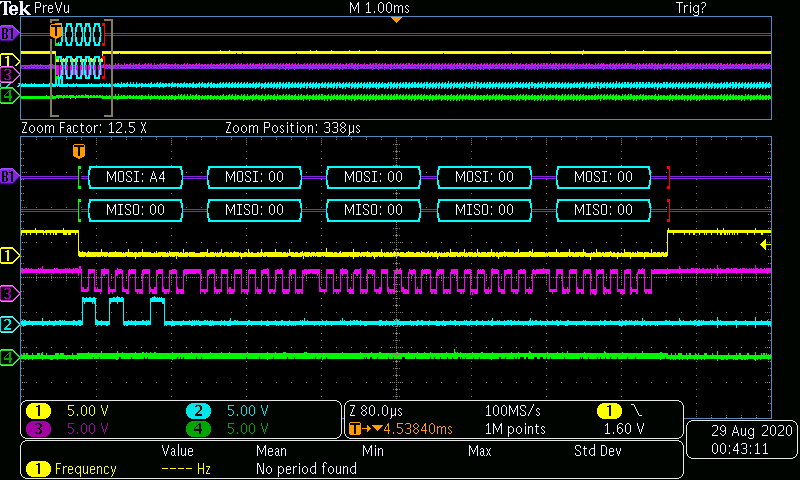
\includegraphics[width = \textwidth]{graphics/TMC4671_TestDrive4}
\caption{Übertragung mit Zoom (Testdrive).}
\label{fig:TMC4671_TestDrive4}
\end{figure}

\begin{figure}[H]
\center
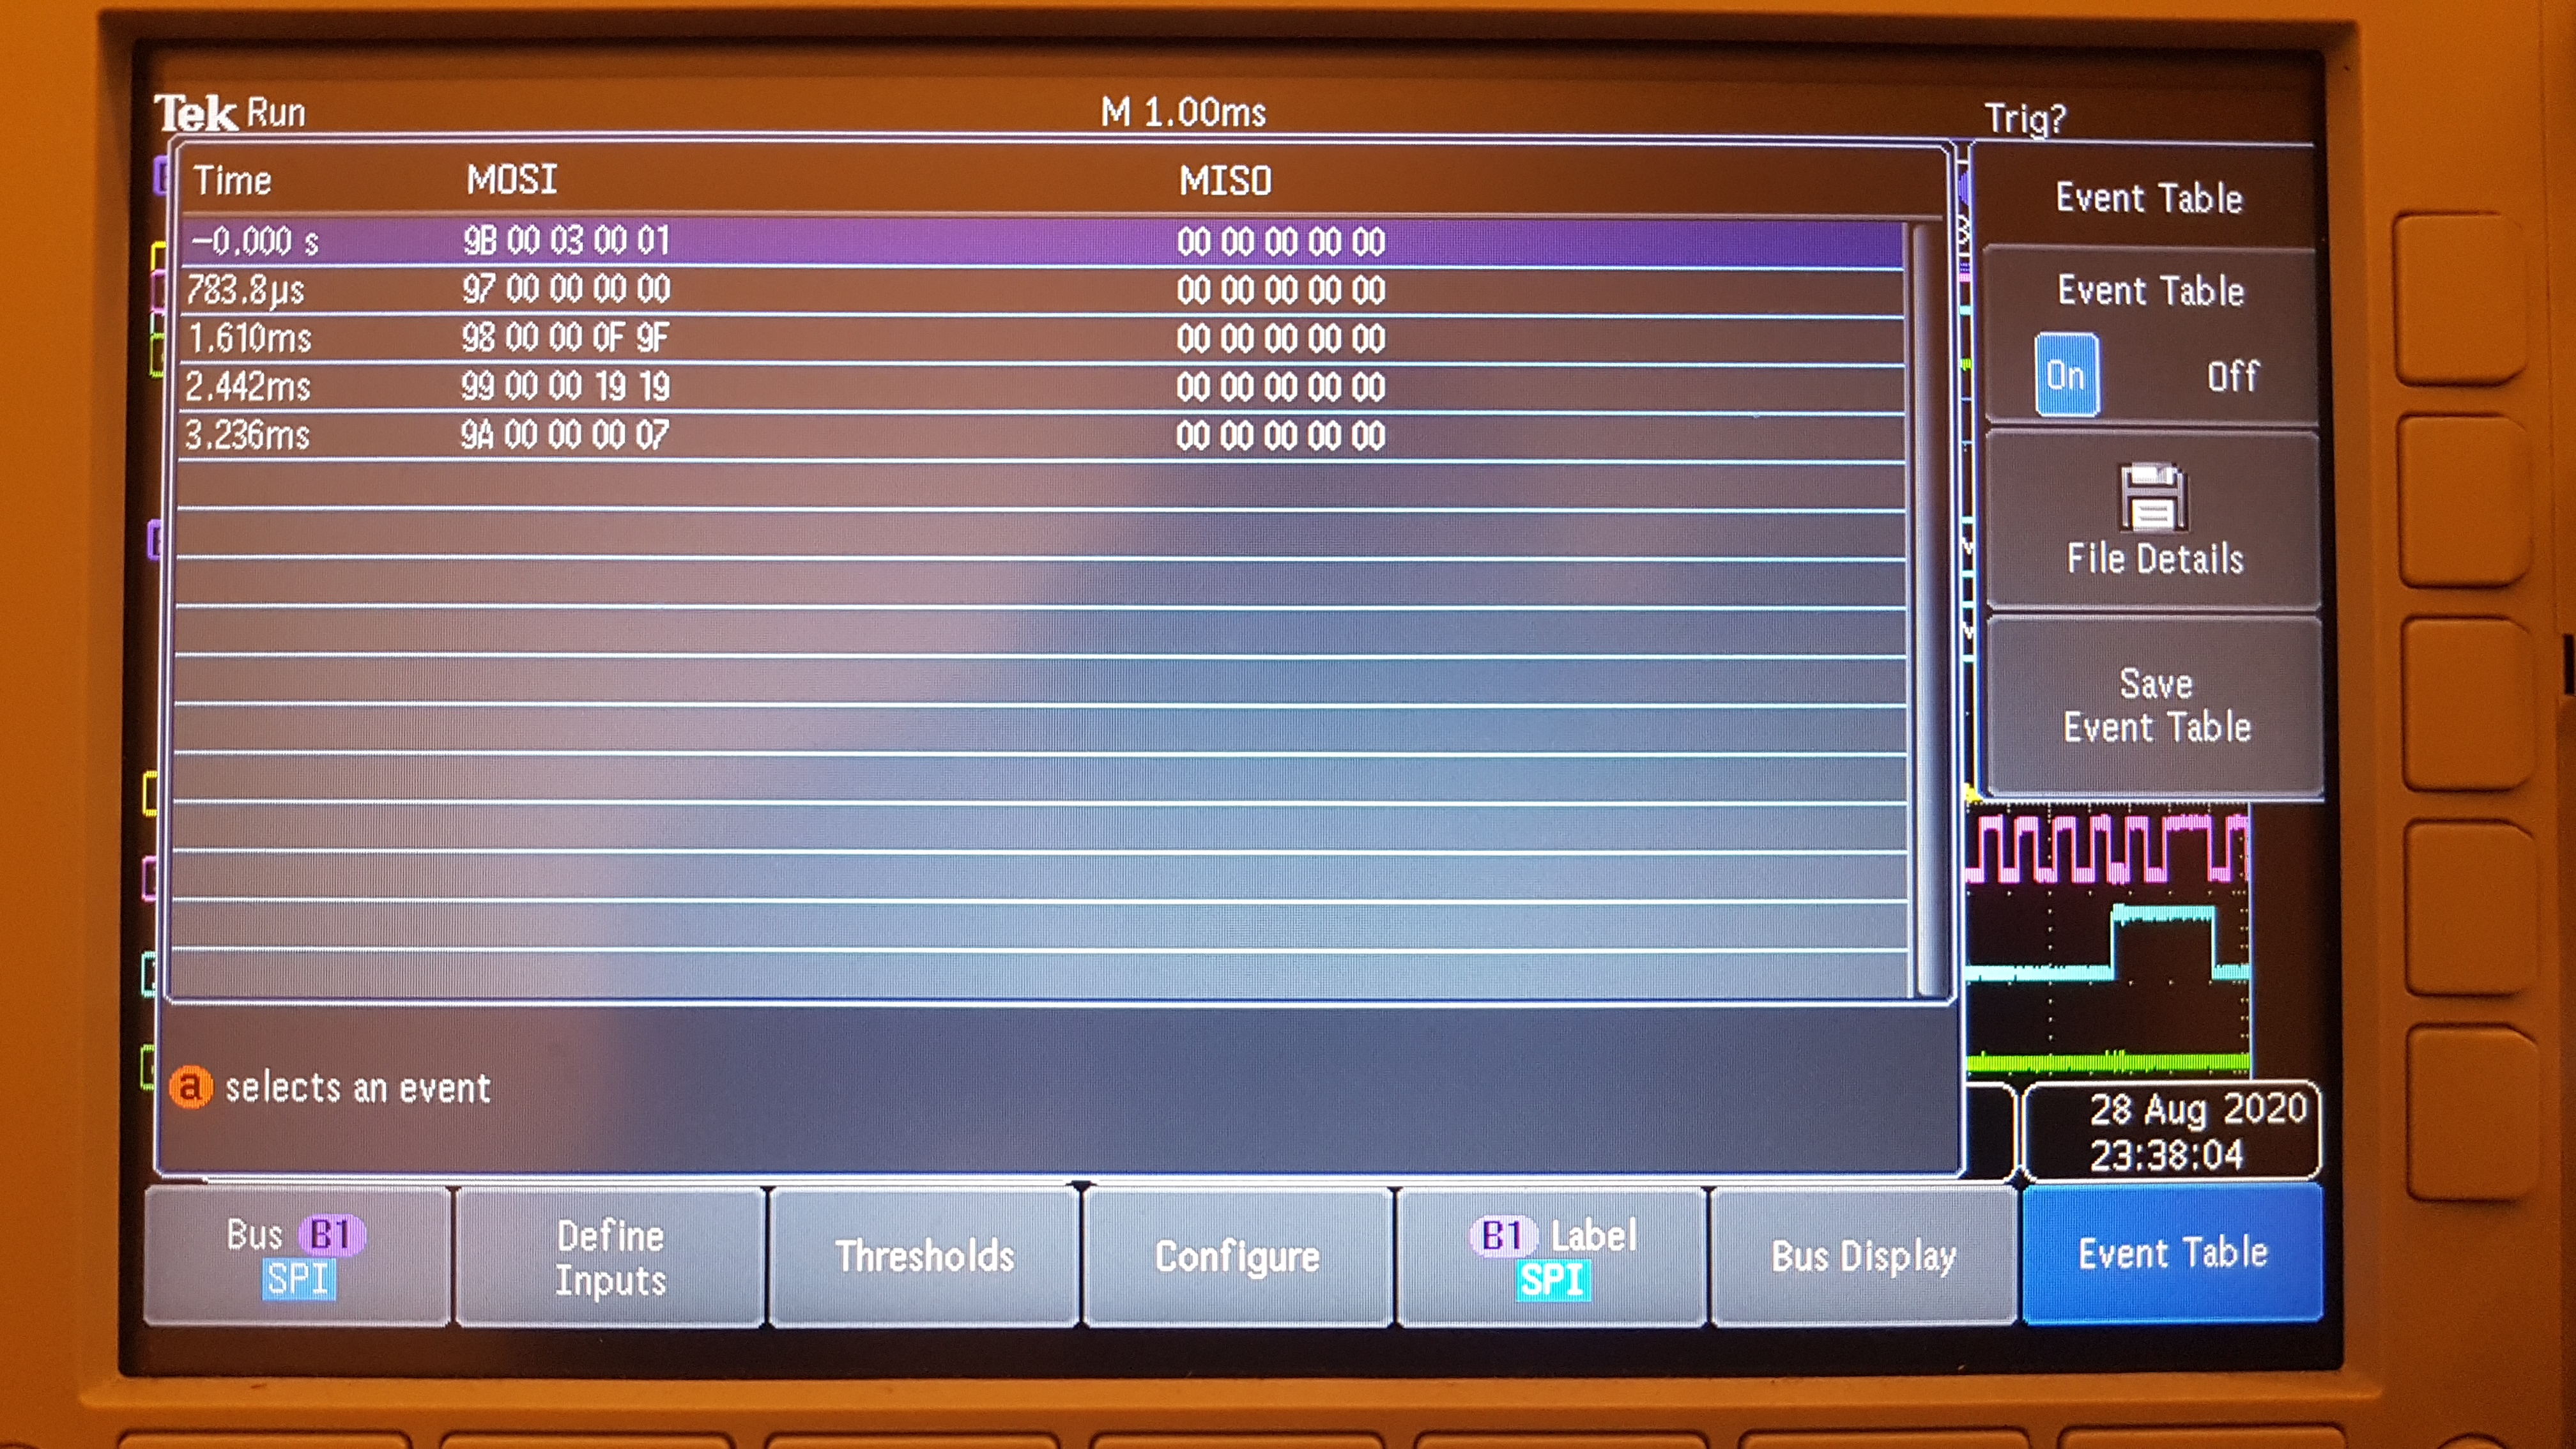
\includegraphics[width = \textwidth]{graphics/TMC4671_TimeTable_Beschreiben1_Bild}
\caption{Event-Table Inbetriebnahme TMC4671.}
\label{fig:TMC4671_TimeTable_Beschreiben1_Bild}
\end{figure}

\begin{figure}[H]
\center
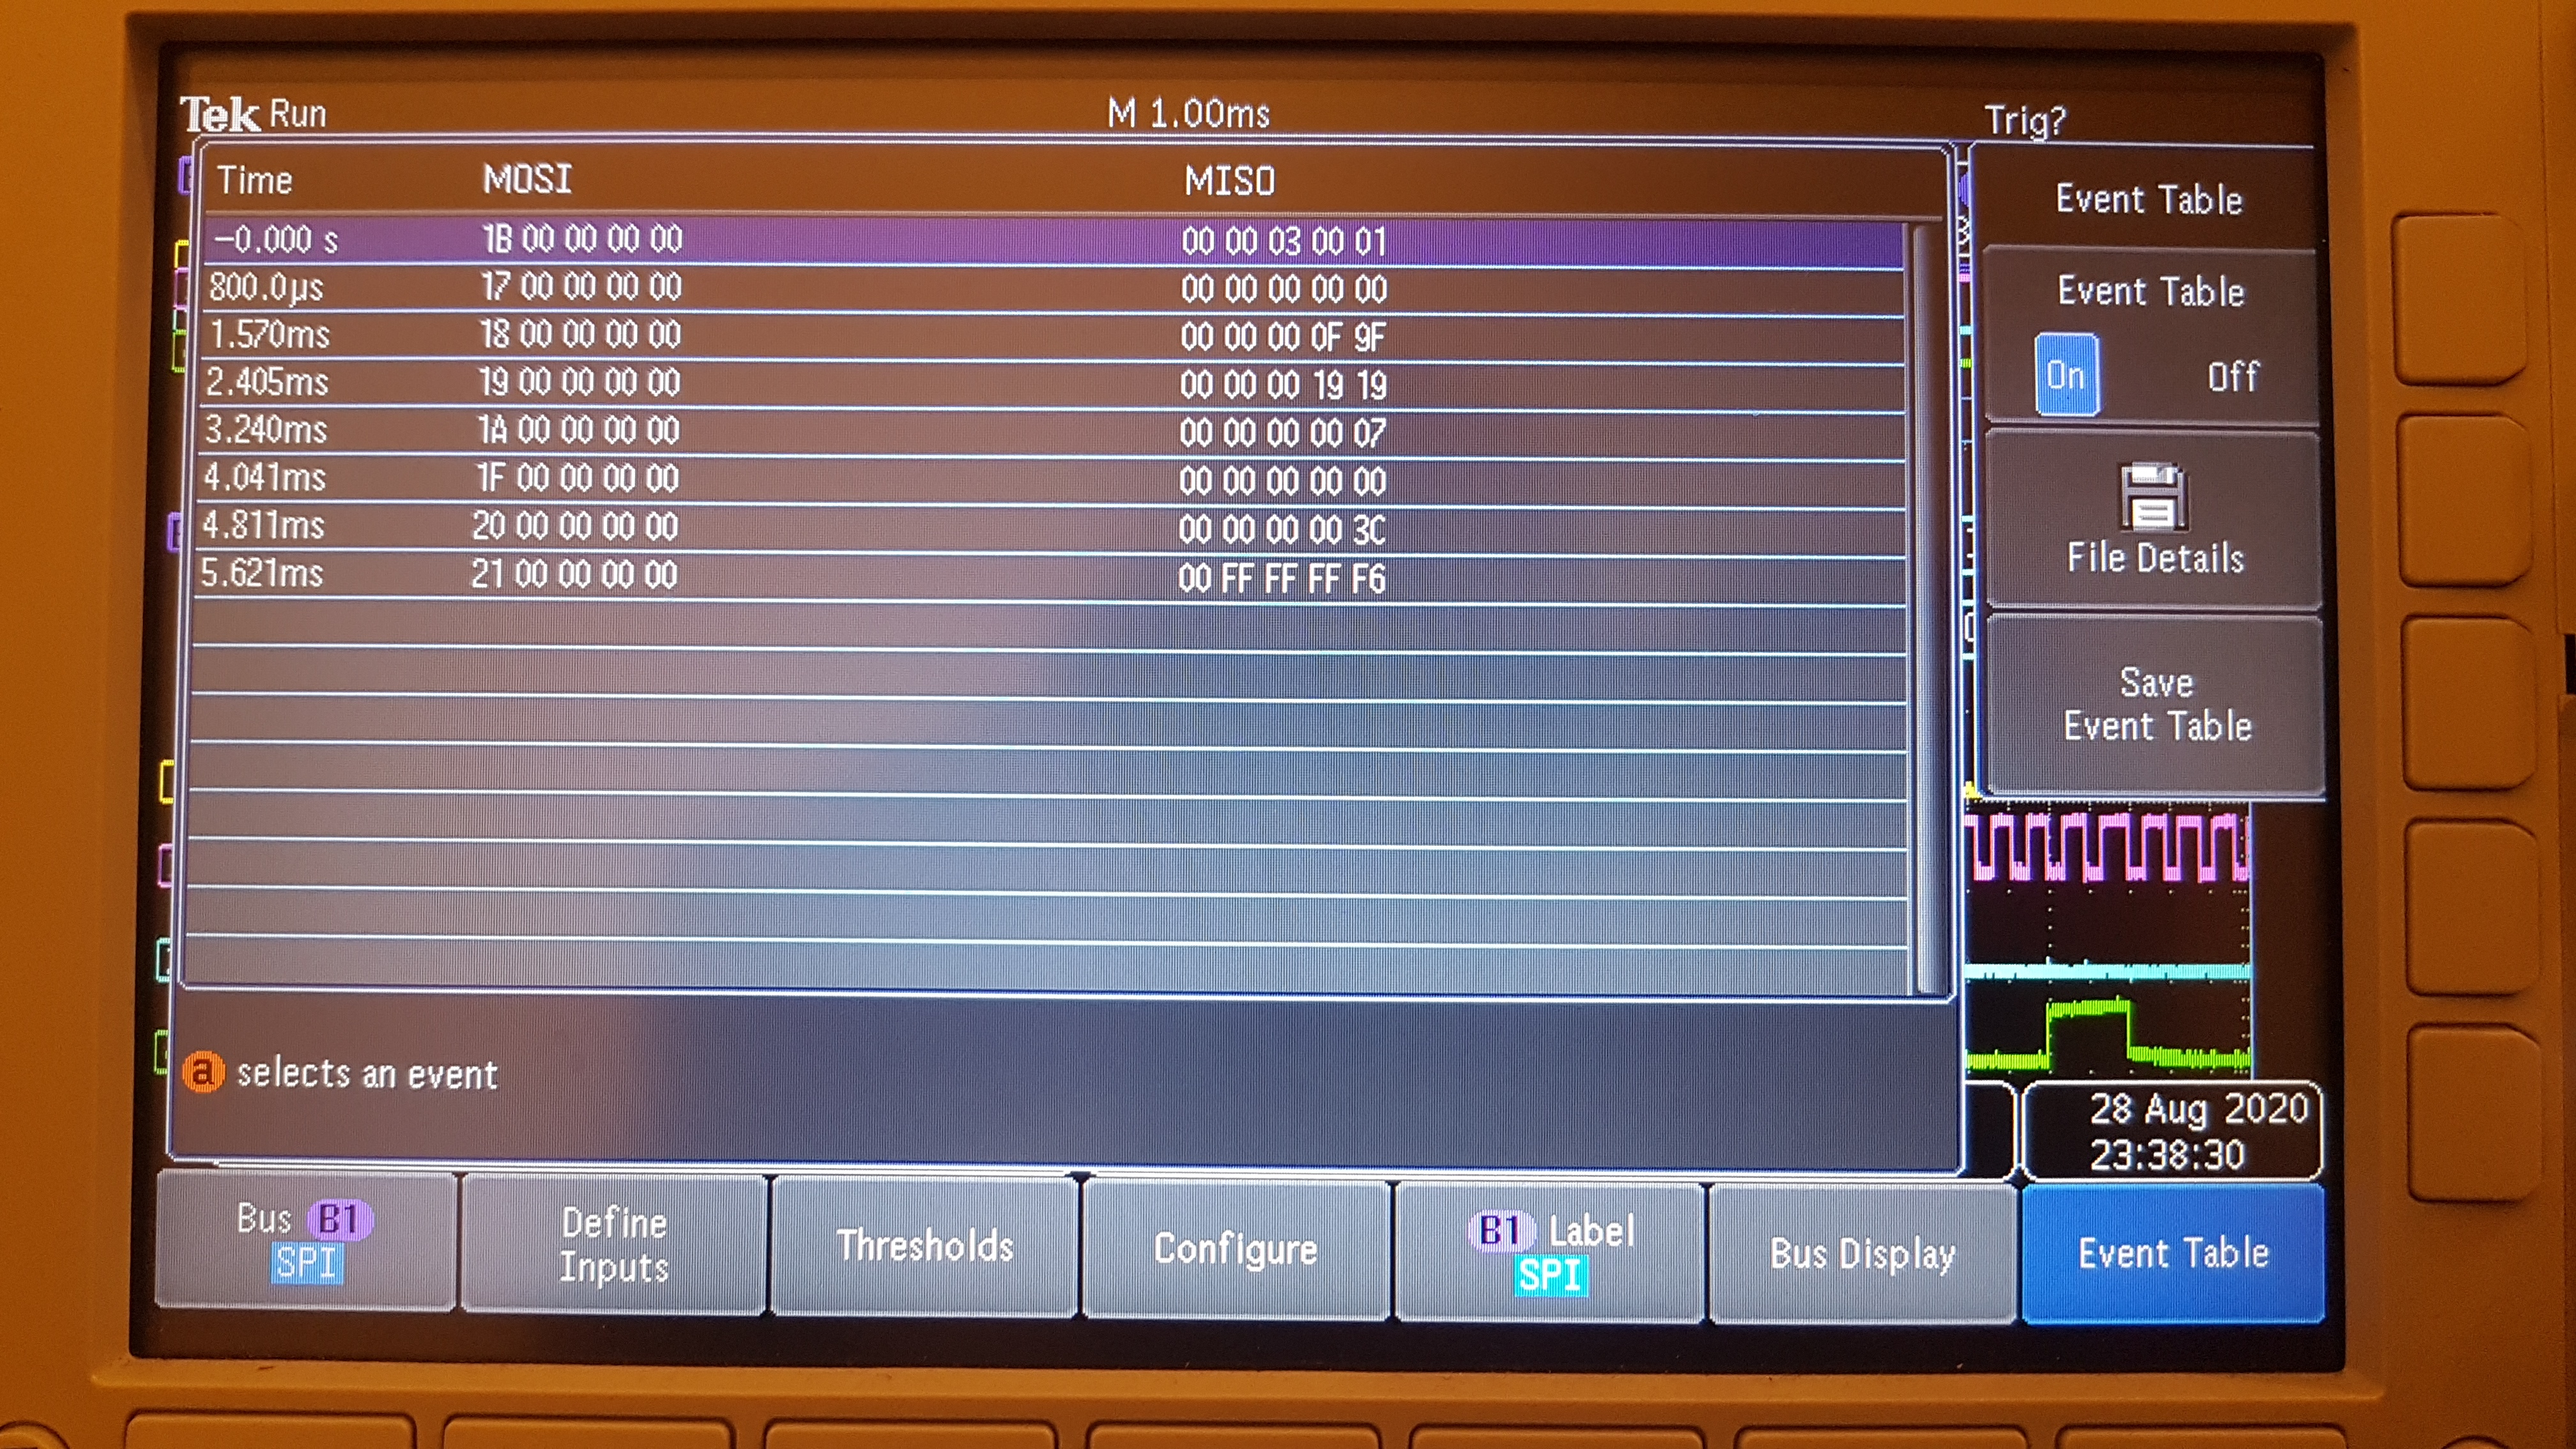
\includegraphics[width = \textwidth]{graphics/TMC4671_TimeTable_Lesen_Bild}
\caption{Event-Table Inbetriebnahme TMC4671.}
\label{fig:TMC4671_TimeTable_Lesen_Bild}
\end{figure}

\newpage

\subsubsection{Inbetriebnahme Gate-Ctrl}\label{Appendix:TMC4671_Gate_Ctrl}

\begin{figure}[H]
\center
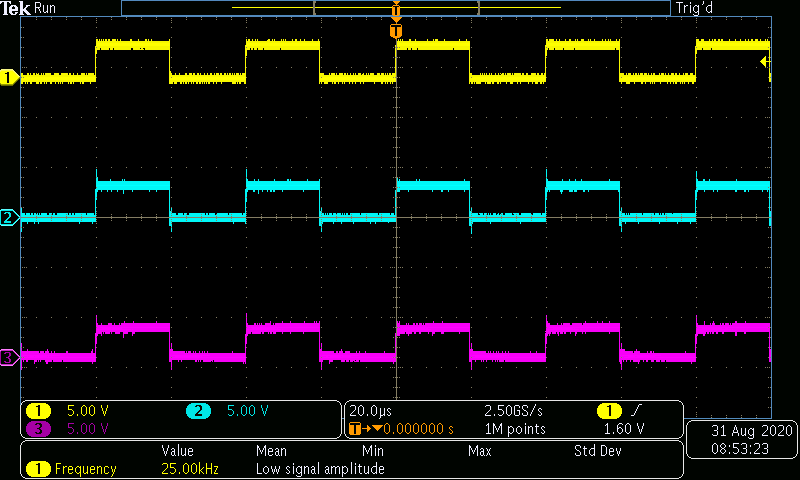
\includegraphics[width = \textwidth]{graphics/TMC4671_Gate_Signal_H}
\caption{Steuersignale PWM 48V. Gelb = U, Blau = V, Magenta = W}
\label{fig:TMC4671_Gate_Signal_H}
\end{figure}

\begin{figure}[H]
\center
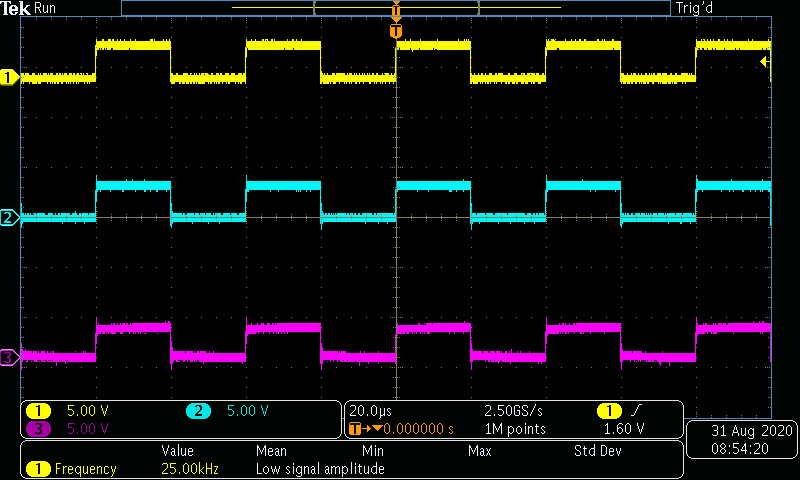
\includegraphics[width = \textwidth]{graphics/TMC4671_Gate_Signal_L}
\caption{Steuersignale PWM 0V. Gelb = U, Blau = V, Magenta = W}
\label{fig:TMC4671_Gate_Signal_L}
\end{figure}